\section{Análisis de interrelaciones}

   \paragraph{}Una vez definidas las distintas entidades presentes en el
   modelo, a continuación se detallarán las distintas relaciones que mantienen
   entre ellas. Las interrelaciones por describir son las siguientes:

   \begin{itemize}
    \item Interrelación Administrador Centro - Centro.
    \item Interrelación Centro - Titulación.
    \item Interrelación Titulación - Asignatura.
    \item Interrelación Asignatura - Asignatura Curso Académico.
    \item Interrelación Alumno - Alumno Curso Académico.
    \item Interrelación Alumno Curso Académico - Calificación Alumno Asignatura CA.
    \item Interrelación Asignatura Curso Académico - Calificación Alumno Asignatura CA.
    \item Interrelación Asesor - Asesor Curso Académico.
    \item Interrelación Departamento - Asesor Curso Académico.
    \item Interrelación Plantilla Entrevista Asesor - Asesor Curso Académico.
    \item Interrelación Plantilla Entrevista Asesor - Pregunta Asesor.
    \item Interrelación Asesor Curso Académico - Alumno Curso Académico.
    \item Interrelación Plantilla Entrevista Oficial - Pregunta Oficial.
    \item Interrelación Alumno Curso Académico - Reunión.
    \item Interrelación Reunión - Pregunta Oficial.
    \item Interrelación Reunión - Pregunta Asesor.
   \end{itemize}

   \paragraph{}Para la descripción de cada relación entre entidades, se
   utilizarán los siguientes apartados:

   \begin{description}
      \item[Definición] Especifica el motivo por el cual se produce la
           interrelación y entre qué tipos de entidad se da lugar.

      \item[Características] En este aparatado se mostrará la siguiente
           información:

            \begin{itemize}
             \item Nombre del tipo de interrelación.
             \item Tipo de la interrelación, es decir, fuerte o débil. En el
                   caso de que sea débil se especifica el tipo de debilidad:
                   existencia o identificación.
             \item Cardinalidad de la interrelación y cardinalidad con la que
                   cada tipo de entidad participa en la interrelación.
             \item Número de atributos del tipo de interrelación.
             \item Posibles restricciones que pueda tener la interrelación, en
                   el caso de que hubiera.
            \end{itemize}

      \item[Diagrama] Representación gráfica del tipo de interrelación.

      \item[Descripción de los atributos] Se describirán cada uno de los
           atributos que forman parte del tipo de interrelación. Para cada uno
           de ellos se indicará lo siguiente:

           \begin{itemize}
            \item Definición del atributo.
            \item Dominio en el cual se encuentra.
            \item Ejemplo práctico de cada atributo.
           \end{itemize}

      \item[Ejemplo práctico del tipo de interrelación] En este apartado se
           muestra una ocurrencia concreta del tipo de interrelación.
   \end{description}

\subsection{Interrelación Administrador Centro - Centro}

   \begin{description}
      \item[Definición] En esta interrelación se deja constancia de que cada
      centro establecido en el sistema dispone, al menos, un administrador de
      centro.

      \item[Características] La interrelación presenta las siguientes
                             características:

         \begin{itemize}
            \item \textbf{Nombre:} AC-C
            \item \textbf{Tipo de la interrelación:} Fuerte
            \item \textbf{Cardinalidad de la interrelación:} N:M
                  \begin{itemize}
                     \item Administrador Centro: administra (0,n)
                     \item Centro: es\_administrado\_por (1,n)
                  \end{itemize}
            \item \textbf{Número de atributos:} Ninguno
         \end{itemize}

      \item[Diagrama] La figura \ref{diagramaAC-C} muestra el diagrama de la
                      interrelación.
      \item \begin{figure}[!ht]
            \begin{center}
            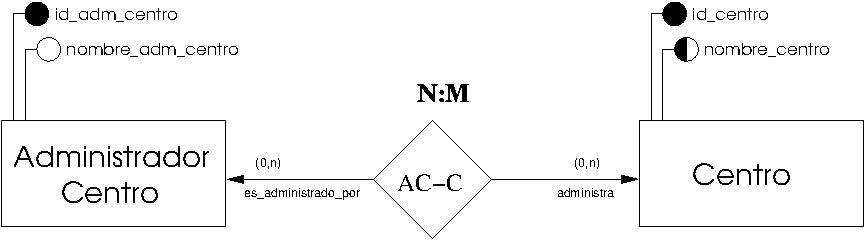
\includegraphics[]{07.Modelo_Entidad-Interrelacion/7.3.Analisis_Interrelaciones/diagramas/AC-C.pdf}
            \caption{Diagrama de la interrelación AC-C.}
            \label{diagramaAC-C}
            \end{center}
         \end{figure}

      \item[Ejemplo práctico del tipo de interrelación]

      \item \begin{center}
            \begin{tabular}{ | c | c | }
            \hline
            \multicolumn{2}{ | c | }{\textbf{Tipo de interrelación AC-C}} \\
            \hline
            \textbf{Administrador Centro} & \textbf{Centro}\\
            \hline
            id\_adm\_centro & id\_centro \\
            \hline
            9 & 15 \\
            \hline
            \end{tabular}
         \end{center}

   \end{description}

\subsection{Interrelación Centro - Titulación}

   \begin{description}
      \item[Definición]

      \item[Características] La interrelación presenta las siguientes
                             características:

         \begin{itemize}
            \item \textbf{Nombre:}
            \item \textbf{Tipo de la interrelación:}
            \item \textbf{Cardinalidad de la interrelación:}
            \item \textbf{Número de atributos:}
         \end{itemize}

      \item[Diagrama] La figura \textit{RELLENAR} muestra el diagrama de la
                      interrelación.

      \item[Descripción de los atributos]

      \item[Ejemplo práctico del tipo de interrelación]
   \end{description}

\subsection{Interrelación Titulación - Asignatura}

   \begin{description}
      \item[Definición] En esta interrelación se deja constancia de que cada
      titulación establecida en el sistema podrá disponer de varias asignaturas.

      \begin{itemize}
       \item Una titulación puede disponer de varias asignaturas.
       \item Una asignatura solamente puede pertenecer a una determinada
             titulación.
      \end{itemize}

      \item[Características] La interrelación presenta las siguientes
                             características:

         \begin{itemize}
            \item \textbf{Nombre:} T-A
            \item \textbf{Tipo de la interrelación:} El tipo de entidad
                  Asignatura es débil por identificación respecto al tipo de
                  entidad Titulación.
            \item \textbf{Cardinalidad de la interrelación:} 1:N
                  \begin{itemize}
                     \item Titulación: dispone\_de (0,n)
                     \item Asignatura: pertenece\_a (1,1)
                  \end{itemize}
            \item \textbf{Número de atributos:} Ninguno.
         \end{itemize}

      \item[Diagrama] La figura \ref{diagramaT-A} muestra el diagrama de la
                      interrelación.

      \item \begin{figure}[!ht]
            \begin{center}
            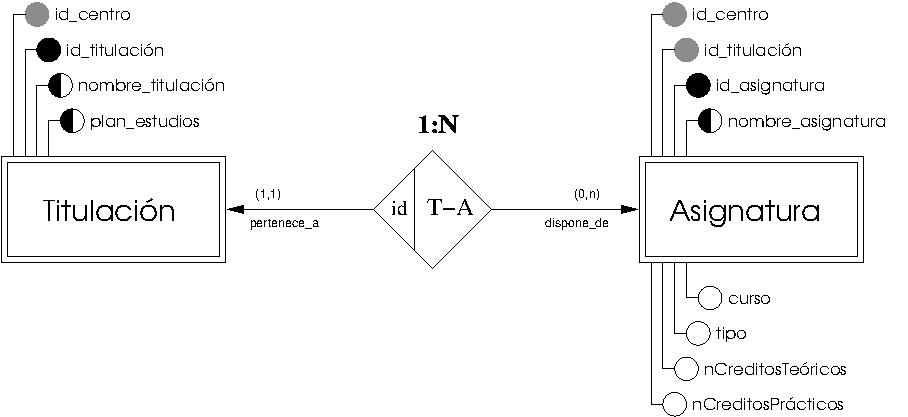
\includegraphics[]{07.Modelo_Entidad-Interrelacion/7.3.Analisis_Interrelaciones/diagramas/T-A.pdf}
            \caption{Diagrama de la interrelación T-A.}
            \label{diagramaT-A}
            \end{center}
         \end{figure}

      \item[Ejemplo práctico del tipo de interrelación]

      \item \begin{center}
            \begin{tabular}{ | r r | }
            \hline
            \multicolumn{2}{ | c | }{\textbf{Tipo de interrelación T-A}} \\
            \hline
            \textbf{Titulación} & \\
            id\_centro & 15 \\
            id\_titulación & 3 \\
            \hline
            \textbf{Asignatura} & \\
            id\_centro & 15 \\
            id\_titulación & 3 \\
            id\_asignatura & 17 \\
            \hline
            \end{tabular}
         \end{center}
   \end{description}

\subsection{Interrelación Asignatura - Asignatura Curso Académico}

   \begin{description}
      \item[Definición]

      \item[Características] La interrelación presenta las siguientes
                             características:

         \begin{itemize}
            \item \textbf{Nombre:}
            \item \textbf{Tipo de la interrelación:}
            \item \textbf{Cardinalidad de la interrelación:}
            \item \textbf{Número de atributos:}
         \end{itemize}

      \item[Diagrama] La figura \textit{RELLENAR} muestra el diagrama de la
                      interrelación.

      \item[Descripción de los atributos]

      \item[Ejemplo práctico del tipo de interrelación]
   \end{description}

\subsection{Interrelación Alumno - Alumno Curso Académico}

   \begin{description}
      \item[Definición] En esta interrelación se deja constancia de que un
      alumno puede estar matriculado durante un número indeterminado de cursos
      académicos.

      \item[Características] La interrelación presenta las siguientes
                             características:

         \begin{itemize}
            \item \textbf{Nombre:} A-AlCA
            \item \textbf{Tipo de la interrelación:} El tipo de entidad
                  Alumno Curso Académico es débil por identificación respecto al
                  tipo de entidad Alumno.
            \item \textbf{Cardinalidad de la interrelación:} 1:N
                  \begin{itemize}
                     \item Alumno: matriculado\_en (0,n)
                     \item Alumno Curso Académico: es\_un (1,1)
                  \end{itemize}
            \item \textbf{Número de atributos:} Ninguno.
         \end{itemize}

      \item[Diagrama] La figura \ref{diagramaA-AlCA} muestra el diagrama de la
                      interrelación.

      \item \begin{figure}[!ht]
            \begin{center}
            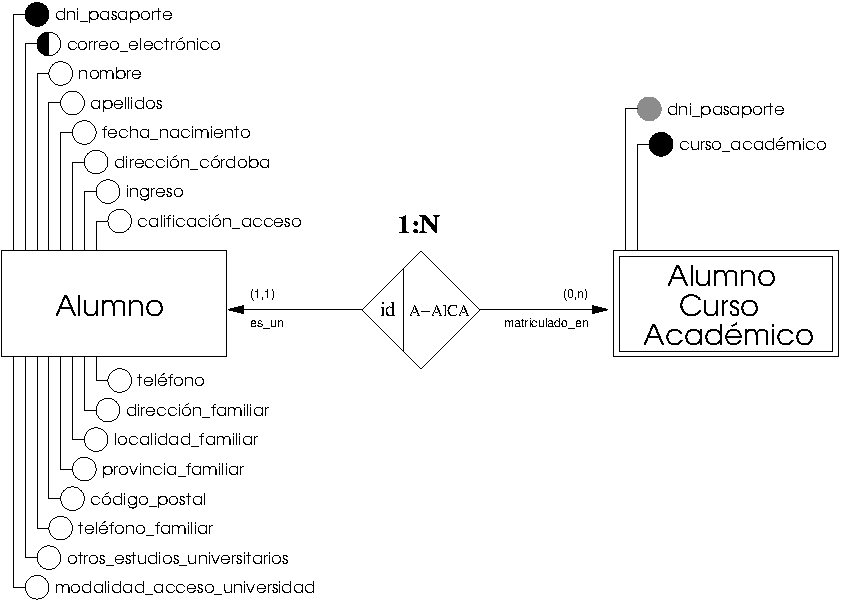
\includegraphics[]{07.Modelo_Entidad-Interrelacion/7.3.Analisis_Interrelaciones/diagramas/A-AlCA.pdf}
            \caption{Diagrama de la interrelación A-AlCA.}
            \label{diagramaA-AlCA}
            \end{center}
         \end{figure}

      \item[Ejemplo práctico del tipo de interrelación]

      \item \begin{center}
            \begin{tabular}{ | r r | }
            \hline
            \multicolumn{2}{ | c | }{\textbf{Tipo de interrelación A-AlCA}} \\
            \hline
            \textbf{Alumno} & \\
            dni\_pasaporte & 01234567A \\
            \hline
            \textbf{Alumno Curso Académico} & \\
            dni\_pasaporte & 01234567A \\
            curso\_académico & 2008 \\
            \hline
            \end{tabular}
         \end{center}
   \end{description}

\subsection{Interrelación Alumno Curso Académico - Calificación Alumno
            Asignatura CA}

   \begin{description}
      \item[Definición] En esta interrelación se deja constancia de que un
      alumno obtendrá una calificación de una asignatura en una determinada
      convocatoria durante un curso académico.

      \begin{itemize}
       \item Un \textit{Alumno Curso Académico} puede tener varias
             \textit{Calificación Alumno Asignatura CA}.
       \item Una \textit{Calificación Alumno Asignatura CA} solamente puede
             pertenecer a un \textit{Alumno Curso Académico}.
      \end{itemize}

      \item[Características] La interrelación presenta las siguientes
                             características:

         \begin{itemize}
            \item \textbf{Nombre:} AlCA-Cal
            \item \textbf{Tipo de la interrelación:} El tipo de entidad
                  Calificación Alumno Asignatura CAes débil por identificación
                  respecto al tipo de entidad Alumno Curso Académico.
            \item \textbf{Cardinalidad de la interrelación:} 1:N
                  \begin{itemize}
                     \item Alumno Curso Académico: tiene (0,n)
                     \item Calificación Alumno Asignatura CA: pertenece\_a (1,1)
                  \end{itemize}
            \item \textbf{Número de atributos:} Ninguno.
         \end{itemize}

      \item[Diagrama] La figura \ref{diagramaAlCA-Cal} muestra el diagrama de la
                      interrelación.

      \item \begin{figure}[!ht]
            \begin{center}
            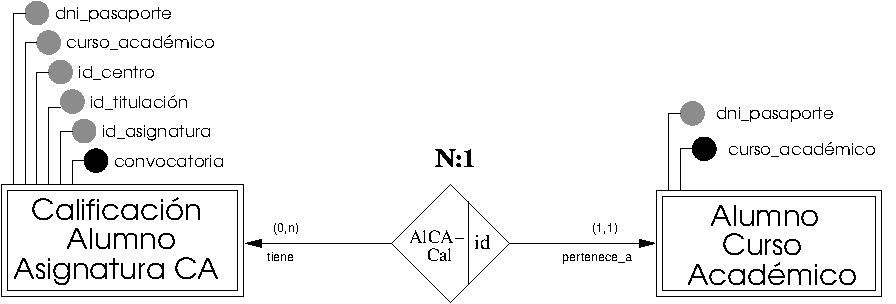
\includegraphics[]{07.Modelo_Entidad-Interrelacion/7.3.Analisis_Interrelaciones/diagramas/AlCA-Cal.pdf}
            \caption{Diagrama de la interrelación AlCA-Cal.}
            \label{diagramaAlCA-Cal}
            \end{center}
         \end{figure}

      \item[Ejemplo práctico del tipo de interrelación]

      \item \begin{center}
            \begin{tabular}{ | r r | }
            \hline
            \multicolumn{2}{ | c | }{\textbf{Tipo de interrelación AlCA-Cal}} \\
            \hline
            \textbf{Alumno Curso Académico} & \\
            dni\_pasaporte & 01234567A \\
            curso\_académico & 2008 \\
            \hline
            \textbf{Calificación Alumno Asignatura CA} & \\
            dni\_pasaporte & 01234567A \\
            curso\_académico & 2008 \\
            id\_centro & 15 \\
            id\_titulación & 3\\
            id\_asignatura & 17\\
            convocatoria & febrero \\
            \hline
            \end{tabular}
         \end{center}
   \end{description}

\subsection{Interrelación Asignatura Curso Académico - Calificación Alumno
            Asignatura CA}

   \begin{description}
      \item[Definición] En esta interrelación se deja constancia de que un
      alumno obtendrá una calificación de una asignatura en una determinada
      convocatoria durante un curso académico.

      \begin{itemize}
       \item Una \textit{Asignatura Curso Académico} puede tener varias
             \textit{Calificación Alumno Asignatura CA}.
       \item Una \textit{Calificación Alumno Asignatura CA} solamente puede
             pertenecer a una \textit{Asignatura Curso Académico}.
      \end{itemize}

      \item[Características] La interrelación presenta las siguientes
                             características:

         \begin{itemize}
            \item \textbf{Nombre:} ACA-Cal
            \item \textbf{Tipo de la interrelación:} El tipo de entidad
                  Calificación Alumno Asignatura CAes débil por identificación
                  respecto al tipo de entidad Alumno Curso Académico.
            \item \textbf{Cardinalidad de la interrelación:} 1:N
                  \begin{itemize}
                     \item Asignatura Curso Académico: tiene (0,n)
                     \item Calificación Alumno Asignatura CA: pertenece\_a (1,1)
                  \end{itemize}
            \item \textbf{Número de atributos:} Ninguno.
         \end{itemize}

      \item[Diagrama] La figura \ref{diagramaACA-Cal} muestra el diagrama de la
                      interrelación.

      \item \begin{figure}[!ht]
            \begin{center}
            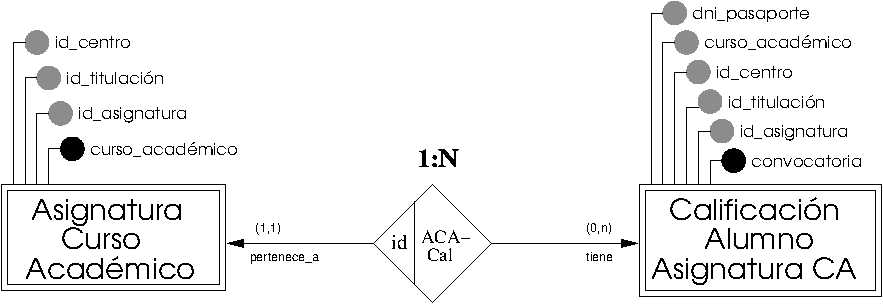
\includegraphics[]{07.Modelo_Entidad-Interrelacion/7.3.Analisis_Interrelaciones/diagramas/ACA-Cal.pdf}
            \caption{Diagrama de la interrelación ACA-Cal.}
            \label{diagramaACA-Cal}
            \end{center}
         \end{figure}

      \item[Ejemplo práctico del tipo de interrelación]

      \item \begin{center}
            \begin{tabular}{ | r r | }
            \hline
            \multicolumn{2}{ | c | }{\textbf{Tipo de interrelación ACA-Cal}} \\
            \hline
            \textbf{Asignatura Curso Académico} & \\
            id\_centro & 15 \\
            id\_titulación & 3\\
            id\_asignatura & 17\\
            curso\_académico & 2008\\
            \hline
            \textbf{Calificación Alumno Asignatura CA} & \\
            dni\_pasaporte & 01234567A \\
            curso\_académico & 2008 \\
            id\_centro & 15 \\
            id\_titulación & 3\\
            id\_asignatura & 17\\
            convocatoria & febrero \\
            \hline
            \end{tabular}
         \end{center}
   \end{description}

\subsection{Interrelación Asesor - Asesor Curso Académico}

   \begin{description}
      \item[Definición] En esta interrelación se deja constancia de que un
      asesor puede ofrecer servicios de asesoría durante distintos cursos
      académicos.

      \begin{itemize}
       \item Un \textit{Asesor} puede asesorar a varios \textit{Asesor Curso Académico}.
       \item Un \textit{Asesor Curso Académico} es un \textit{Asesor}.
      \end{itemize}

      \item[Características] La interrelación presenta las siguientes
                             características:

         \begin{itemize}
            \item \textbf{Nombre:} Ase-AseCA
            \item \textbf{Tipo de la interrelación:} El tipo de entidad
                  Asesor Curso Académico es débil por identificación respecto al
                  tipo de entidad Asesor.
            \item \textbf{Cardinalidad de la interrelación:} 1:N
                  \begin{itemize}
                     \item Asesor: asesora (0,n)
                     \item Asesor Curso Académico: es\_un (1,1)
                  \end{itemize}
            \item \textbf{Número de atributos:} Ninguno.
         \end{itemize}

      \item[Diagrama] La figura \ref{diagramaAse-AseCA} muestra el diagrama de la
                      interrelación.

      \item \begin{figure}[!ht]
            \begin{center}
            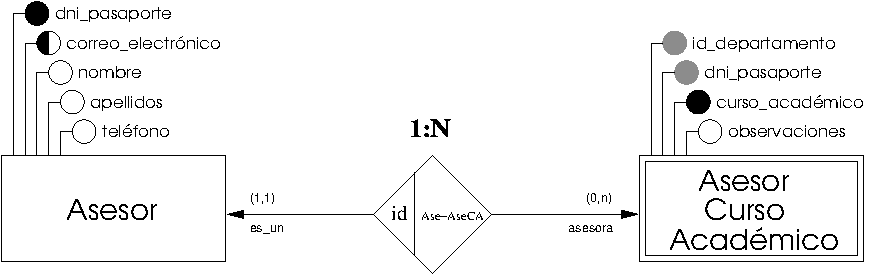
\includegraphics[]{07.Modelo_Entidad-Interrelacion/7.3.Analisis_Interrelaciones/diagramas/Ase-AseCA.pdf}
            \caption{Diagrama de la interrelación Ase-AseCA.}
            \label{diagramaAse-AseCA}
            \end{center}
         \end{figure}

      \item[Ejemplo práctico del tipo de interrelación]

      \item \begin{center}
            \begin{tabular}{ | r r | }
            \hline
            \multicolumn{2}{ | c | }{\textbf{Tipo de interrelación Ase-AseCA}} \\
            \hline
            \textbf{Asesor} & \\
            dni\_pasaporte & 98765432Z \\
            \hline
            \textbf{Asesor Curso Académico} & \\
            dni\_pasaporte & 98765432Z \\
            id\_centro & 2008 \\
            \hline
            \end{tabular}
         \end{center}
   \end{description}

\subsection{Interrelación Departamento - Asesor Curso Académico}

   \begin{description}
      \item[Definición] En esta interrelación se deja constancia de que un
      asesor puede ofrecer servicios de asesoría perteneciendo a un departamento
      durante un determinado curso académico.

      \item[Características] La interrelación presenta las siguientes
                             características:

         \begin{itemize}
            \item \textbf{Nombre:} D-AseCA
            \item \textbf{Tipo de la interrelación:} El tipo de entidad
                  Asesor Curso Académico es débil por existencia respecto al
                  tipo de entidad Departamento.
            \item \textbf{Cardinalidad de la interrelación:} 1:N
            \item \textbf{Número de atributos:} Ninguno.
         \end{itemize}

      \item[Diagrama] La figura \ref{diagramaD-AseCA} muestra el diagrama de la
                      interrelación.

      \item \begin{figure}[!ht]
            \begin{center}
            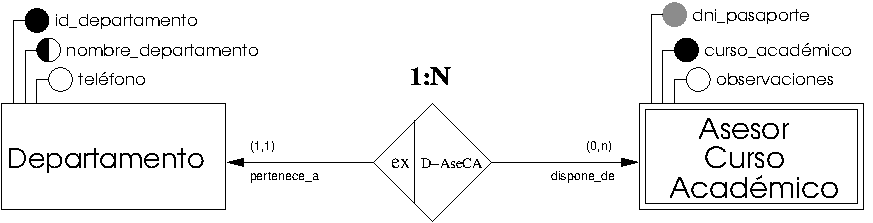
\includegraphics[]{07.Modelo_Entidad-Interrelacion/7.3.Analisis_Interrelaciones/diagramas/D-AseCA.pdf}
            \caption{Diagrama de la interrelación D-AseCA.}
            \label{diagramaD-AseCA}
            \end{center}
         \end{figure}

      \item[Ejemplo práctico del tipo de interrelación]

      \item \begin{center}
            \begin{tabular}{ | r r | }
            \hline
            \multicolumn{2}{ | c | }{\textbf{Tipo de interrelación D-AseCA}} \\
            \hline
            \textbf{Departamento} & \\
            id\_departamento & 22 \\
            \hline
            \textbf{Asesor Curso Académico} & \\
            dni\_pasaporte & 98765432Z \\
            curso\_académico & 2007 \\
            \hline
            \end{tabular}
         \end{center}
   \end{description}

\subsection{Interrelación Plantilla Entrevista Asesor - Asesor Curso Académico}

   \begin{description}
      \item[Definición] En esta interrelación se deja constancia de que un
      usuario asesor puede hacer uso de plantillas de entrevistas de asesor
      durante un determinado curso académico.

      \item[Características] La interrelación presenta las siguientes
                             características:

         \begin{itemize}
            \item \textbf{Nombre:} AseCA-PEA
            \item \textbf{Tipo de la interrelación:} El tipo de entidad
            Plantilla Entrevista Asesor es débil por identificación respecto al
            tipo de entidad Asesor Curso Académico.
            \item \textbf{Cardinalidad de la interrelación:} 1:N
                  \begin{itemize}
                     \item Plantilla Entrevista Asesor: utilizada\_por (1,1)
                     \item Asesor Curso Académico: utiliza (0,n)
                  \end{itemize}
            \item \textbf{Número de atributos:} Ninguno.
         \end{itemize}

      \item[Diagrama] La figura \ref{diagramaPEA-AseCA} muestra el diagrama de
      la interrelación.

      \item \begin{figure}[!ht]
            \begin{center}
            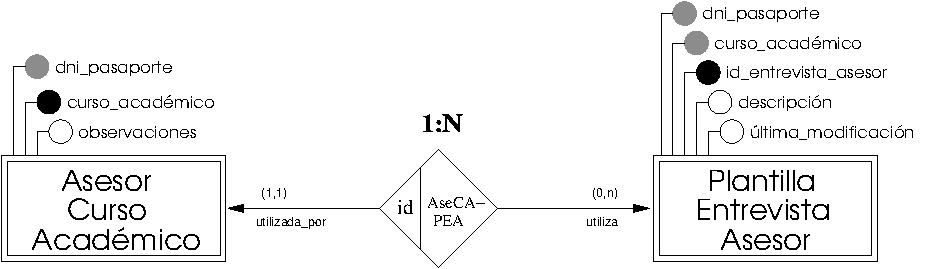
\includegraphics[]{07.Modelo_Entidad-Interrelacion/7.3.Analisis_Interrelaciones/diagramas/PEA-AseCA.pdf}
            \caption{Diagrama de la interrelación PEA-AseCA.}
            \label{diagramaPEA-AseCA}
            \end{center}
         \end{figure}

      \item[Ejemplo práctico del tipo de interrelación]

      \item \begin{center}
            \begin{tabular}{ | r r | }
            \hline
            \multicolumn{2}{ | c | }{\textbf{Tipo de interrelación PEA-AseCA}} \\
            \hline
            \textbf{Plantilla Entrevista Asesor} & \\
            dni\_pasaporte & 98765432Z \\
            curso\_académico & 2008 \\
            id\_entrevista\_asesor & 36 \\
            \hline
            \textbf{Asesor Curso Académico} & \\
            dni\_pasaporte & 98765432Z \\
            curso\_académico & 2008 \\
            \hline
            \end{tabular}
         \end{center}
   \end{description}

\subsection{Interrelación Plantilla Entrevista Asesor - Pregunta Asesor}

   \begin{description}
      \item[Definición] En esta interrelación se deja constancia de que una
      plantilla de entrevista de asesor puede estar compuesta por varias
      preguntas de asesor.

      \item[Características] La interrelación presenta las siguientes
                             características:

         \begin{itemize}
            \item \textbf{Nombre:} PEA-PA
            \item \textbf{Tipo de la interrelación:} El tipo de entidad Pregunta
                  Asesor es débil por identificación respecto al tipo de
                  entidad Plantilla Entrevista Asesor.
            \item \textbf{Cardinalidad de la interrelación:} 1:N
                  \begin{itemize}
                     \item Plantilla Entrevista Asesor: contiene (0,n)
                     \item Pregunta Asesor: forma\_parte\_de (1,1)
                  \end{itemize}
            \item \textbf{Número de atributos:} Ninguno.
         \end{itemize}

      \item[Diagrama] La figura \ref{diagramaPEA-PA} muestra el diagrama de la
                      interrelación.

      \item \begin{figure}[!ht]
            \begin{center}
            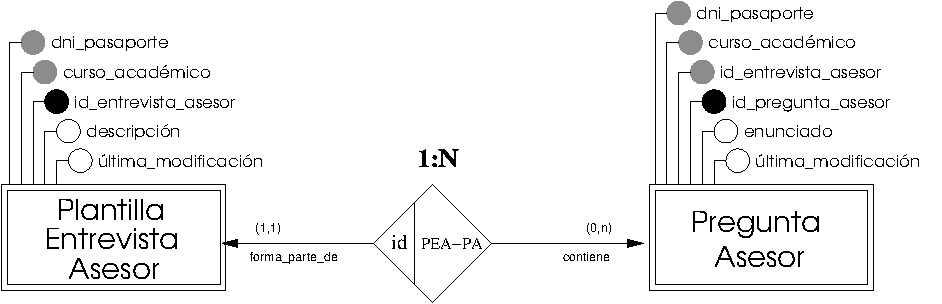
\includegraphics[]{07.Modelo_Entidad-Interrelacion/7.3.Analisis_Interrelaciones/diagramas/PEA-PA.pdf}
            \caption{Diagrama de la interrelación PEA-PA.}
            \label{diagramaPEA-PA}
            \end{center}
         \end{figure}

      \item[Ejemplo práctico del tipo de interrelación]

      \item \begin{center}
            \begin{tabular}{ | r r | }
            \hline
            \multicolumn{2}{ | c | }{\textbf{Tipo de interrelación PEA-PA}} \\
            \hline
            \textbf{Plantilla Entrevista Asesor} & \\
            dni\_pasaporte & 98765432Z \\
            curso\_académico & 2008 \\
            id\_entrevista\_asesor & 36 \\
            \hline
            \textbf{Pregunta Asesor} & \\
            dni\_pasaporte & 98765432Z \\
            curso\_académico & 2008 \\
            id\_entrevista\_asesor & 36 \\
            id\_pregunta\_asesor & 72 \\
            \hline
            \end{tabular}
         \end{center}
   \end{description}

\subsection{Interrelación Asesor Curso Académico - Alumno Curso Académico}

   \begin{description}
      \item[Definición] En esta interrelación se deja constancia de que un
      asesor puede ofrecer servicios de asesoría a un número indeterminado de
      alumnos matriculados durante un determinado curso académico.

      \item[Características] La interrelación presenta las siguientes
                             características:

         \begin{itemize}
            \item \textbf{Nombre:} AseCA-AlCA
            \item \textbf{Tipo de la interrelación:} El tipo de entidad
                  Alumno Curso Académico es débil por existencia respecto al
                  tipo de entidad Asesor Curso Académico.
            \item \textbf{Cardinalidad de la interrelación:} 1:N
                  \begin{itemize}
                     \item Asesor Curso Académico: asesora\_a (0,n)
                     \item Alumno Curso Académico: es\_asesorado\_por (1,1)
                  \end{itemize}
            \item \textbf{Número de atributos:} Ninguno.
            \item \textbf{Restricciones:} Los atributos
                   \textit{curso\_académico} de cada una de las dos entidades
                   que participan en esta interrelación deben tener el mismo
                   valor, por la propia naturaleza de dicha interrelación.
         \end{itemize}

      \item[Diagrama] La figura \ref{diagramaAseCA-AlCA} muestra el diagrama de
                      la interrelación.

       \item \begin{figure}[!ht]
            \begin{center}
            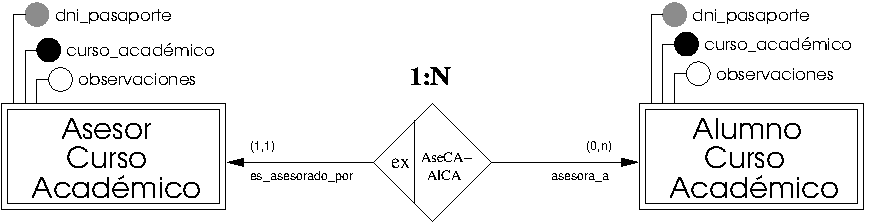
\includegraphics[]{07.Modelo_Entidad-Interrelacion/7.3.Analisis_Interrelaciones/diagramas/AseCA-AlCA.pdf}
            \caption{Diagrama de la interrelación AseCA-AlCA.}
            \label{diagramaAseCA-AlCA}
            \end{center}
         \end{figure}

      \item[Ejemplo práctico del tipo de interrelación]

      \item \begin{center}
            \begin{tabular}{ | r r | }
            \hline
            \multicolumn{2}{ | c | }{\textbf{Tipo de interrelación AseCA-AlCA}} \\
            \hline
            \textbf{Asesor Curso Académico} & \\
            dni\_pasaporte & 98765432Z \\
            curso\_académico & 2008 \\
            \hline
            \textbf{Alumno Curso Académico} & \\
            dni\_pasaporte & 01234567A \\
            curso\_académico & 2008 \\
            \hline
            \end{tabular}
         \end{center}
   \end{description}

\subsection{Interrelación Plantilla Entrevista Oficial - Pregunta Oficial}

   \begin{description}
      \item[Definición] En esta interrelación se deja constancia de que una
      plantilla de entrevista oficial puede estar compuesta por varias preguntas
      oficiales.

      \item[Características] La interrelación presenta las siguientes
                             características:

         \begin{itemize}
            \item \textbf{Nombre:} PEO-PO
            \item \textbf{Tipo de la interrelación:} El tipo de entidad Pregunta
                  Oficial es débil por identificación respecto al tipo de
                  entidad Plantilla Entrevista Oficial.
            \item \textbf{Cardinalidad de la interrelación:} 1:N
                  \begin{itemize}
                     \item Plantilla Entrevista Oficial: contiene (0,n)
                     \item Pregunta Oficial: forma\_parte\_de (1,1)
                  \end{itemize}
            \item \textbf{Número de atributos:} Ninguno.
         \end{itemize}

      \item[Diagrama] La figura \ref{diagramaPEO-PO} muestra el diagrama de la
                      interrelación.

      \item \begin{figure}[!ht]
            \begin{center}
            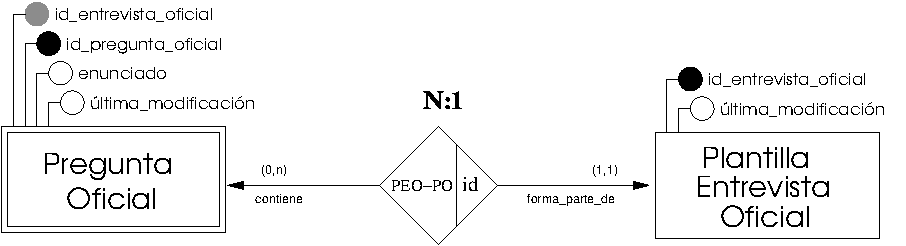
\includegraphics[]{07.Modelo_Entidad-Interrelacion/7.3.Analisis_Interrelaciones/diagramas/PEO-PO.pdf}
            \caption{Diagrama de la interrelación PEO-PO.}
            \label{diagramaPEO-PO}
            \end{center}
         \end{figure}

      \item[Ejemplo práctico del tipo de interrelación]

      \item \begin{center}
            \begin{tabular}{ | r r | }
            \hline
            \multicolumn{2}{ | c | }{\textbf{Tipo de interrelación PEO-PO}} \\
            \hline
            \textbf{Plantilla Entrevista Oficial} & \\
            id\_entrevista\_oficial & 24 \\
            \hline
            \textbf{Pregunta Oficial} & \\
            id\_entrevista\_oficial & 24 \\
            id\_pregunta\_oficial & 55 \\
            \hline
            \end{tabular}
         \end{center}
   \end{description}

\subsection{Interrelación Alumno Curso Académico - Reunión}

   \begin{description}
      \item[Definición] En esta interrelación se deja constancia de que un
      alumno puede participar en reuniones con su asesor durante un determinado
      curso académico.

      \item[Características] La interrelación presenta las siguientes
                             características:

         \begin{itemize}
            \item \textbf{Nombre:} AlCA-R
            \item \textbf{Tipo de la interrelación:} El tipo de entidad Reunión
                  es débil por identificación respecto al tipo de entidad Alumno
                  Curso Académico .
            \item \textbf{Cardinalidad de la interrelación:} 1:N
                  \begin{itemize}
                     \item Alumno Curso Académico: participa\_en (0,n)
                     \item Reunión: realizada\_a (1,1)
                  \end{itemize}
            \item \textbf{Número de atributos:} Ninguno.
         \end{itemize}

      \item[Diagrama] La figura \ref{diagramaAlCA-R} muestra el diagrama de la
                      interrelación.

      \item \begin{figure}[!ht]
            \begin{center}
            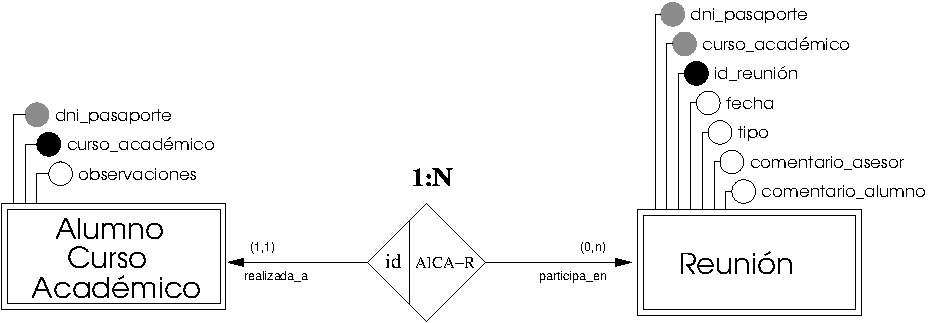
\includegraphics[]{07.Modelo_Entidad-Interrelacion/7.3.Analisis_Interrelaciones/diagramas/AlCA-R.pdf}
            \caption{Diagrama de la interrelación AlCA-R.}
            \label{diagramaAlCA-R}
            \end{center}
         \end{figure}

      \item[Ejemplo práctico del tipo de interrelación]

      \item \begin{center}
            \begin{tabular}{ | r r | }
            \hline
            \multicolumn{2}{ | c | }{\textbf{Tipo de interrelación AlCA-R}} \\
            \hline
            \textbf{Alumno Curso Académico} & \\
            dni\_pasaporte & 01234567A \\
            curso\_académico & 2008 \\
            \hline
            \textbf{Reunión} & \\
            dni\_pasaporte & 98765432Z \\
            curso\_académico & 2008 \\
            id\_reunión & 121 \\
            fecha & 01/01/2009 \\
            tipo & Individual \\
            \hline
            \end{tabular}
         \end{center}
   \end{description}

\subsection{Interrelación Reunión - Pregunta Oficial}

   \begin{description}
      \item[Definición] En esta interrelación se deja constancia de que una
      reunión puede estar compuesta por varias preguntas oficiales.

      \item[Características] La interrelación presenta las siguientes
                             características:

         \begin{itemize}
            \item \textbf{Nombre:} R-PO
            \item \textbf{Tipo de la interrelación:} Fuerte.
            \item \textbf{Cardinalidad de la interrelación:} N:M
                  \begin{itemize}
                     \item Reunión: compuesta\_por (0,n)
                     \item Pregunta Oficial: aparece\_en (0,n)
                  \end{itemize}
            \item \textbf{Número de atributos:} Uno: respuesta.
         \end{itemize}

      \item[Diagrama] La figura \ref{diagramaR-PO} muestra el diagrama de la
                      interrelación.

      \item \begin{figure}[!ht]
            \begin{center}
            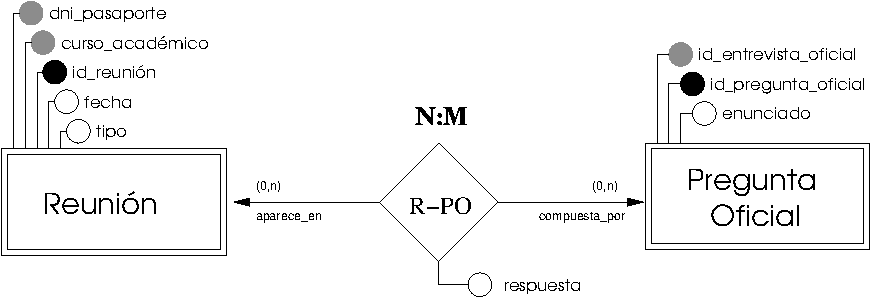
\includegraphics[]{07.Modelo_Entidad-Interrelacion/7.3.Analisis_Interrelaciones/diagramas/R-PO.pdf}
            \caption{Diagrama de la interrelación R-PO.}
            \label{diagramaR-PO}
            \end{center}
         \end{figure}

      \item[Descripción de los atributos] La interrelación presenta el
      siguiente atributo:

       \begin{itemize}
        \item \textbf{respuesta}
          \begin{itemize}
            \item \textbf{Definición:} Establece la contestación del alumno a la
            pregunta realizada.
            \item \textbf{Dominio:} Conjunto de caracteres alfanuméricos.
            \item \textbf{Carácter:} Obligatorio.
            \item \textbf{Ejemplo práctico:} Antiguo alumno.
            \item \textbf{Información adicional:} El dato lo introduce el
            usuario alumno al contestar a la pregunta realizada.
         \end{itemize}
       \end{itemize}

      \item[Ejemplo práctico del tipo de interrelación]

      \item \begin{center}
            \begin{tabular}{ | r r | }
            \hline
            \multicolumn{2}{ | c | }{\textbf{Tipo de interrelación R-PO}} \\
            \hline
            \textbf{Reunión} & \\
            dni\_pasaporte & 98765432Z \\
            curso\_académico & 2008 \\
            id\_reunión & 121 \\
            fecha & 01/01/2009 \\
            tipo & Individual \\
            \hline
            \textbf{Pregunta Oficial} & \\
            id\_entrevista\_oficial & 24 \\
            id\_pregunta\_oficial & 55 \\
            enunciado & ¿Quién le ha informado de esta carrera? \\
            \hline
            \textbf{Atributos} & \\
            respuesta & Antiguo alumno \\
            \hline
            \end{tabular}
         \end{center}
   \end{description}

\subsection{Interrelación Reunión - Pregunta Asesor}

   \begin{description}
      \item[Definición] En esta interrelación se deja constancia de que una
      reunión puede estar compuesta por varias preguntas de asesor.

      \begin{itemize}
       \item Una \textit{Reunión} puede estar compuesta por varias
             \textit{Pregunta Asesor}.
       \item Una \textit{Pregunta Asesor} puede aparecer en varias
             \textit{Reunión}.
      \end{itemize}

      \item[Características] La interrelación presenta las siguientes
                             características:

         \begin{itemize}
            \item \textbf{Nombre:} R-PA
            \item \textbf{Tipo de la interrelación:} Fuerte.
            \item \textbf{Cardinalidad de la interrelación:} N:M
                  \begin{itemize}
                     \item Reunión: compuesta\_por (0,n)
                     \item Pregunta Oficial: aparece\_en (0,n)
                  \end{itemize}
            \item \textbf{Número de atributos:} Uno: respuesta.
            \item \textbf{Restricciones:} Debido a que existe un ciclo en el
                  modelo Entidad-Relación planteado (ver la figura
                  \ref{diagramaER} ) que afecta a las entidades \textit{Alumno
                  Curso Académico}, \textit{Asesor Curso Académico},
                  \textit{Plantilla Entrevista Asesor}, \textit{Pregunta Asesor}
                  y \textit{Reunión}, no es posible controlar que un determinado
                  \textit{Alumno Curso Académico} tenga reuniones exclusivamente
                  con las \textit{Pregunta Asesor} de su \textit{Asesor Curso
                  Académico}, por lo que será necesario controlar este
                  comportamiento mediante la lógica de la aplicación.
         \end{itemize}

      \item[Diagrama] La figura \ref{diagramaR-PA} muestra el diagrama de la
                      interrelación.

      \item \begin{figure}[!ht]
            \begin{center}
            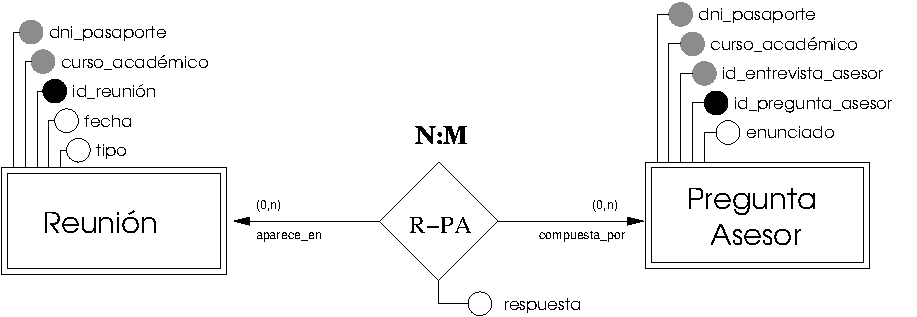
\includegraphics[]{07.Modelo_Entidad-Interrelacion/7.3.Analisis_Interrelaciones/diagramas/R-PA.pdf}
            \caption{Diagrama de la interrelación R-PA.}
            \label{diagramaR-PA}
            \end{center}
         \end{figure}

      \item[Descripción de los atributos] La interrelación presenta el
      siguiente atributo:

       \begin{itemize}
        \item \textbf{respuesta}
          \begin{itemize}
            \item \textbf{Definición:} Establece la contestación del alumno a la
            pregunta realizada.
            \item \textbf{Dominio:} Conjunto de caracteres alfanuméricos.
            \item \textbf{Carácter:} Obligatorio.
            \item \textbf{Ejemplo práctico:} Antiguo alumno.
            \item \textbf{Información adicional:} El dato lo introduce el
            usuario alumno al contestar a la pregunta realizada.
         \end{itemize}
       \end{itemize}

      \item[Ejemplo práctico del tipo de interrelación]

      \item \begin{center}
            \begin{tabular}{ | r r | }
            \hline
            \multicolumn{2}{ | c | }{\textbf{Tipo de interrelación R-PA}} \\
            \hline
            \textbf{Reunión} & \\
            dni\_pasaporte & 98765432Z \\
            curso\_académico & 2008 \\
            id\_reunión & 121 \\
            \hline
            \textbf{Pregunta Asesor} & \\
            dni\_pasaporte & 98765432Z \\
            curso\_académico & 2008 \\
            id\_entrevista\_asesor & 36 \\
            id\_pregunta\_asesor & 72 \\
            enunciado & Nivel de inglés \\
            \hline
            \textbf{Pregunta Asesor} & \\
            respuesta & Alto \\
            \hline
            \end{tabular}
         \end{center}
   \end{description}

